\chapter{Evaluación experimental}
\label{cap:evaluacionexperimental}

Se hace una introducción.

\section{Predicción de tiempo de respuesta a transacción de lectura}
\label{evaluacionexperimental:ptrq}

Se hace una breve introducción al cpaítulo anterior. 

Se menciona los resultados obtenidos con la regresión, se dice que no se tuvieron muy buenos resultados con la regresión, se deja a ver por qué no se obtuvieron muy buenos resultados (índice con los que se hicieron experimentos, consultas, etc.).

\subsection{Predictor perfecto}
\label{evaluacionexperimental:predictorperfecto}

Decir que no es el foco de esta tesi, que los resultados obtenidos no fueron muy buenos s y que para evaluar los algoritmos de scheduling  también se usará un predictor perfecto. Decir cómo se obtuvo un predictor perfecto y ojalá mostrar algún algoritmo.


\section{Wand multithreaded}
\label{evaluacionexperimental:wm}

Introducción al capítulo anterior, dos esquemas, etc. Decir cómo se llevaron a cabo los experimentos, datos que se utilizaron (o quizás decirlos una sola vez). 


\subsection{Wand heap compartido}
\label{evaluacionexperimental:whc}

Se habla un poco de las ventajas que se tenía con este esquema nuevamente, qué se hizo para la implementación, cómo se programó, etc. 

Se muestra el código y ojalá se muestra algún flujo de ejecución para una query específica.
\lstinputlisting[language=C++]{code/TopKMultithreadWandOperatorLocal.h}

Se muestra un gráfico y tabla de eficiencia.


\begin{figure}[!ht]
\centering
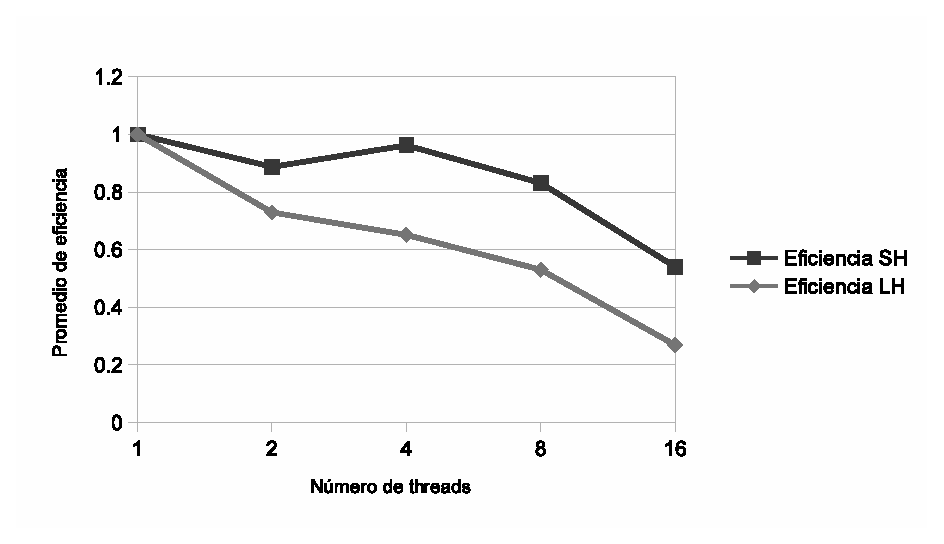
\includegraphics[scale=.75]{images/eficiencia_wand.eps}
\caption{Eficiencias para Wand con heaps compartido y locales}
\label{fig:wand-heap-local}
\end{figure}


\subsection{Wand heap local}
\label{evaluacionexperimental:whl}

Se habla un poco de las ventajas que se tenía con este esquema nuevamente, qué se hizo para la implementación, cómo se programó, etc. 

Se muestra el código y ojalá se muestra algún flujo de ejecución para una query específica.

Se muestra un gráfico y tabla de eficiencia.

Meter algo para comparar ambos enfoques en un mismo gráfico o algo así. (no se si sea buena idea tener dos gráficos de eficiencia o solo 1).


\section{Estrategias de scheduling}
\label{evaluacionexperimental:estrategiasscheduling}

Hablar separado cada una de ellas, mostrando implementación y cómo se llevaron a cabo los experimentos.

1. Comparar las tres estrategias de scheduling (decir que TimesRanges es mejor) ==> Con predictor perfecto también?
2. Comparar TimesRanges con baseline ==> Con Predictor perfecto también.  
4. Decir los problemas que existen en cada una de las estrategias que se pierden tiempos.
3. Sacar a la luz la nueva unidades de trabajo ==> Predictor perfecto también.
4. Comparación unidades de trabajo - baseline - TimesRanges.

Conclusiones para cada uno de los gráficos realizados. 


